\chapter{基于多传感器的无人机引导系统设计}

\section{基于激光反射器的引导系统设计}

使用波长为940nm的半导体激光器,功率为25w,发出连续照明用激光,具体参数见错误!未找到引用源。。在无人机平台前端安装全反射棱镜,使用无觇牌对中杆棱镜ADH11-S,它是仿Topcon角锥棱镜,正面加常数-30mm,背面加常数0mm。全反射棱镜保证了各个方向的光都会按照原方向反射回去,即从转台发射的940nm激光会按照原来方向回到原点。同时,在可见光相机前安装940nm窄带滤光片,使可见光相机只能收到940nm波长的光。

本系统选用山东神戎电子股份有限公司生产的SHR-JLI1000激光照明器,该设备主要分为940mm激光的产生和940mm激光的发射两个部分,如图 9所示,(a)为激光器的产生部件,(b)为激光器的发射部件,激光器的发射部件可以调节激光出射的照明角度,通过调节这个角度可以对目标实现远距离和近距离的有效探测识别,激光器的发射部件同样可以和激光器的产生部件分开,可以方便的安装在需要的位置上。

\section{红外相机传感器}
红外热像仪是利用红外探测器和光学成像物镜接受被测目标的红外辐射能量,将分布图形反映到红外探测器的光敏元件上,从而获得红外热像图,这种热像图与物体表面的热场分布相对应。通俗地讲红外热像仪就是将物体发出的不可见红外能量转变为可见的热图像,如图 7所示,主要的参数指标如下。
本系统选用的浙江大力科技股份有限公司生产的红外热像仪CM6240FC,大气能见度大于10km,相对湿度小于$80\%$,目标与背景温差3K条件下,对3m×3m目标,探测距离不小于7km,识别距离不小于5km。对1.7m×0.5m目标(人),探测距离不小于5km,识别距离不小于2.5km。
最宽视场(40mm焦距):13.75°× 11°;
窄视场(240mm焦距):2.3°× 1.8°;
连续变焦,变焦过程中保持图像清晰;
视场公差:$±5\%$

在红外相机成像后的激光点成像简单,背景噪声小的特点,采用简单的Hough圆提取方式即可实现对目标的跟踪和识别,其基本识别流程图如图\ref{fig:chp06_02_laser_point_detect}所示。
\begin{figure}[!th]
	\centering
	\includegraphics[width=1.0\textwidth]{figs/chp06/chp06_02_laser_point_detect.pdf}	
	\caption{激光照射点的目标识别与跟踪方法}
	\label{fig:chp06_02_laser_point_detect}
\end{figure}

Hough变换(Hough Transform)是由Hough Paul于1962年在一份专利报告中提出\cite{vc1962method}
由保罗·霍夫在1962年提出的Hough变换是一种比较经典的检测不同形状的方法,在由激光主动成像与全反射棱镜配合得到的图像中,目标是以圆形亮斑呈现的,因此本文在对图像进行Canny边缘提取之后,使用Hough变换从中提取出目标所呈现的圆形。

\section{基于超宽带雷达的引导系统设计}

超宽带无线测距以其高距离的分辨力、强穿透力、低截获率以及很强的抗干扰能力在军事、商业等领域得到越来越多的关注。使用的UWB型号为Time Domain公司的PulsONP410,是P400s的升级版本,可通过加载定向天线增大探测距离(http://www.timedomain.com)。实物如图 11所示。

P410的RF传输频率3.1 GHz 到5.3 GHz,中心频率位于4.3 GHz附近;具有两路用户可调天线端口;单个板子尺寸为7.6 x 8.0 x 1.6 cm;可进入睡眠模式,降低功耗;脉冲发射功率可调,可达10Hz以下。该设备探测距离2km以上,如果选用增强型的定向天线探测距离可以达到5km以上,增强型的定向天线如图12所示。加入定向天线后,UWB的探测波半角为20°,当远距离无人机进入探测窗口时,UWB可以探测到目标。UWB的精度为0.5m,当无人机距离目标500m、水平位置为10m,高度为30m时。水平方向的误差为0.01m,高度为0.03m,满足系统的精度要求。

UWB采用应答的方式接收数据,如图13所示,当地面引导系统把地面的请求发给无人机上的UWB时,无人机上的UWB响应地面请求发送数据,地面上的UWB接收这个信息转化为距离信息。该方式有效的解决了一对一的模式,有利于目标远距离的探测,保证了数据的稳定可靠性。传输频率3.1 GHz 到5.3 GHz,因此UWB不易被干扰。

由于DGPS和UWB的天线安装位置不同,且二者天线极化方式不同,进而导致DGPS和UWB的距离解算值存在偏差,因此需要DGPS和UWB联合标定。图 50所示为DGPS与UWB的坐标之间的关系。假设无人机降落过程中的姿态基本保持平稳,通过将无人机分别放置在跑道$400\ m$和$1000\ m$之间,分别记录各个位置的DGPS坐标值和UWB距离值,通过最小二乘法优化即可解算出DGPS和UWB的固定偏差值。

\begin{figure}[!tb]
	\centering
	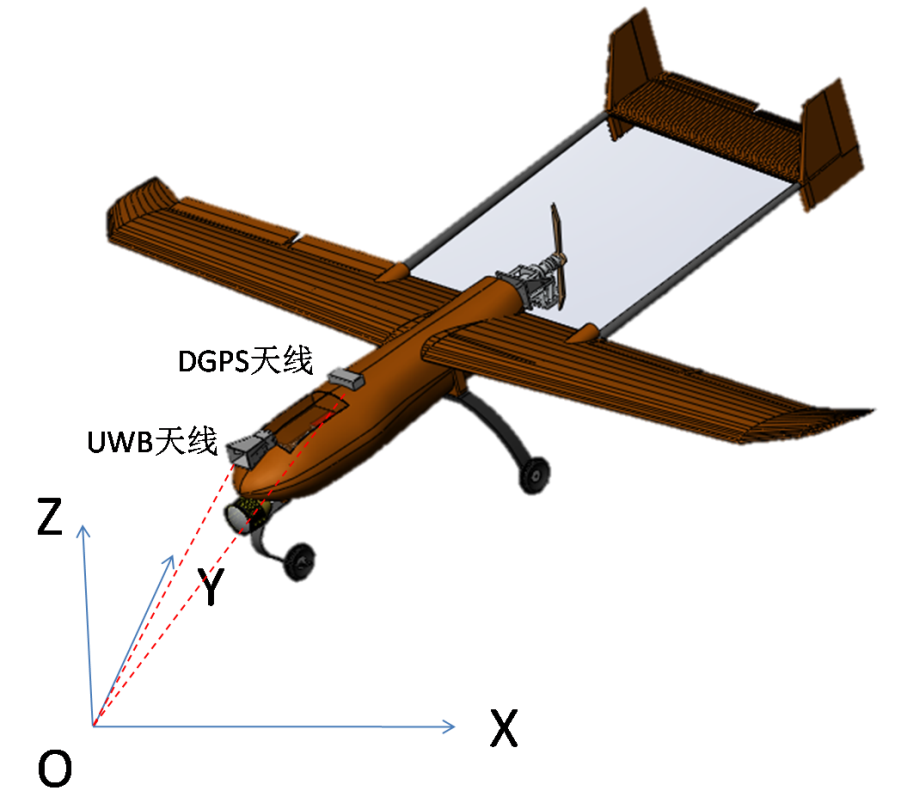
\includegraphics[width=0.5\textwidth]{figs/chp06/chp06_01_UWB_DGPS.pdf}	
	\caption{DGPS与UWB的安装初始偏差示意图}
	\label{fig:chp06_01_UWB_DGPS}
\end{figure}





\section{基于EKF的转台信息滤波问题}
位姿估计问题(Pose Estimation)是估计特定物体相对于参考坐标系的位置和姿态。在传统方法中,GPS、惯性测量单元(IMU)、视觉、激光雷达等作为主要传感器来对目标进行估计和判断。位子估计问题既可以只依赖视觉传感器,也可以综合应用各类型传感器采集到的数据通过滤波得到。在以视觉信息为主的位姿估计方法中,主要有一下两类方法:(1)单目视觉。单视觉方法主要依赖对平面的检测、合作标志的检测、海天线或地平面的检测。(2)多目视觉。多目视觉方法主要指针对特征点在不同成像平面的位置,通过多个相机的排布,从而解算出目标的位置和姿态信息。

基于视觉的位姿估计问题主要应用于人机交互(Human Computer Interaction)、视觉里程计(VO)和器人导航和实时定位与建图(SLAM)。其中,视觉里程计主要通过对系列连续图像进行处理,结合飞行器自身携带的各类传感器,最终得到可靠的三维信息(3D motion)。针对长基线系统,利用EKF方法,将转台信息和图像信息相融合,可以得到较好的目标位置状态。定义$X$是状态模型
\begin{equation}
X=[Pos^s, V^s, C^{Att}, w^{Att}]^T
\end{equation}
其中
$$
Pos^s=\left[\begin{array}{c}
x_l\\
y_l\\
z_l\\
\end{array}\right],
V^s=\left[\begin{array}{c}
v_x\\
v_y\\
v_z\\
\end{array}\right]
$$
$$
C^{Att}=\left[\begin{array}{c}
lpan\\
ltilt\\
rpan\\
rtilt\\
\end{array}\right],
w^{Att}=\left[\begin{array}{c}
wlpan\\
wltilt\\
wrpan\\
wrtilt\\
\end{array}\right].
$$
上述所有变量均在世界坐标系下,其中$lpan$ 和 $ltilt$ 表示左侧相机的俯仰角度和水平角度; $rpan$ 和 $rtilt$ 对应右侧相机的两个角度; $wlpan, wltilt, wrpan, wrtilt$ 表示上述四个角度的角速度。
在第$k$次迭代过程中,状态转换方程如下
\begin{equation}
\bar{x}_{k|k_1}=F_k\bar{x}_{k-1|k-1}
\end{equation}
其中$F_k$是状态转换矩阵。根据EKF的基本假设,在第$k$时刻的状态只从第$k-1$时刻得到。因此可以得到目标的预测位置和相机的姿态解算公式,
\begin{equation}
\overline{Pos}^s_{k|k-1}=\Delta t V^s_{k-1|k-1} + {Pos}^s_{k-1|k-1}
\end{equation}
\begin{equation}
\overline{C}^{Att}_{k|k-1}=\Delta t w^{Att}_{k-1|k-1} + \overline{C}^{Att}s_{k-1|k-1}
\end{equation}
其中$\Delta t$表示相邻两次时间间隔。状态转换方程可以写为,
\begin{equation}
\bar{x}_{k|k-1}=\left[\begin{matrix}
I_{3\times 3} & \Delta t_{3\times 3} & \textbf{0}_{3\times 4} & \textbf{0}_{3\times 4}\\
\textbf{0}_{3\times 3} & I_{3\times 3} & \textbf{0}_{3\times 4} & \textbf{0}_{3\times 4}\\
\textbf{0}_{4\times 3} & \textbf{0}_{4\times 3} & I_{4\times 4} & \Delta t_{4\times 4}\\
\textbf{0}_{4\times 3} & \textbf{0}_{4\times 3} & \textbf{0}_{4\times 4} & I_{4\times 4}\\
\end{matrix}\right]\bar{x}_{k-1|k-1}
\end{equation}
其中$\Delta t_{n \times n}$表示$n \times n$阶矩阵,其对角线位置为$\Delta t$,其余位置为0。在第$k$时刻,系统的协方差矩阵为,
\begin{equation}
P_{k|k-1}=F_kP_{k-1|k-1}F^T_k+G_kQ_kG^T_k
\end{equation}
其中$Q_k$是动态系统的高斯噪声,$G_k$是第$k$时刻$Q_k$的Jacobian矩阵。状态协方差矩阵由四个部分组成,分别对应:目标-目标、目标-相机、相机-相机和相机-目标,其公式为
\begin{equation}
P_k=\left[
\begin{matrix}
P_{T|T} & P_{T|C} \\
P_{C|T} & P_{C|C} \\
\end{matrix}\right].
\end{equation}

EKF的观测模型基于传统的相机成像模型和映射模型,测量向量$z$为,
\begin{equation}
z=[Pos^I_L, Pos^I_R, C^{PTU}]^T
\end{equation} 
其中$Pos^I_L$和$Pos^I_R$分别表示目标在左右相机的位置,$(u^L_k, v^L_k)$和$(u^R_k, v^R_k)$表示目标在相平面的位置。考虑到相机模型为典型的针孔模型,目标位置$\overline{Pos}^s_{k|k-1}$通过转换从世界坐标系到图像坐标系。这里,假设相机光心位置和PTU转台位置在运动过程中保持不变,即忽略安装偏移误差。为了计算目标在相平面的位置,将相机位置、内参数等引入方程,
\begin{equation}
\left[\begin{matrix}
\overline{Pos}^I \\
1\\
\end{matrix}\right]
=h(\overline{Pos}^s_{k|k-1}, \overline{C}^{Att}_{k|k-1})
=\lambda N^{in}\overline{M}^{out}_{k|k-1}\overline{Pos}^s_{k|k-1}
\end{equation}
其中$\lambda$是归一化参数。$N^{in}$和$\overline{M}^{out}_{k|k-1}$是转换矩阵。其他参数可以通过如下方程表达,
\begin{equation}
\overline{M}^{out}_{k|k-1}
= \left[
\begin{matrix}
\bar{R}^c_{k|k-1} & T \\
\textbf{0}^T_3 & 1 \\
\end{matrix}
\right]
\end{equation}
和
\begin{equation}
N^{in}=
\left[
\begin{matrix}
1/d_x & 0 & u_o \\
0 & 1/d_y & v_0 \\
0 & 0 & 1 \\
\end{matrix}
\right]
\left[
\begin{matrix}
f & 0 & 0 & 0 \\
0 & f & 0 & 0 \\
0 & 0 & 0 & 1 \\
\end{matrix}
\right]
\end{equation}
其中$\bar{R}^c_{k|k-1}$是旋转矩阵$\overline{C}^{Att}_{k|k-1}$和$T$表达相机坐标系和世界坐标系之间的位置关系。至此,可以得到观测模型,
\begin{equation}
\bar{z_k}=
\left[
\begin{matrix}
\overline{Pos}^I_L \\
\overline{Pos}^I_R \\
\overline{C}^{PTU} \\
\end{matrix}
\right]
=
\left[
\begin{matrix}
Block (\lambda_L N^{in}_L \overline{M}^{out}_{L(k|k-1)}\overline{Pos}^s_{k|k-1} )\\
Block (\lambda_R N^{in}_R\overline{M}^{out}_{R(k|k-1)}\overline{Pos}^s_{k|k-1}  )\\
I_{4 \times 4}\overline{C}^{Att}_{k|k-1} \\
\end{matrix}
\right]
\end{equation}
定义$Block(\cdot)$作为仅提取矩阵前两项的函数。


$x_k$是$z_k$的更新结果。根据观测模型$h$,其Jacobian矩阵$H_k$可以表达为
\begin{equation}
H_k=\frac{\partial h ( \overline{Pos}^S_{k|k-1}, \overline{C}^{Att}_{k|k-1} )}{\partial x_k} 
\end{equation}
得到卡尔曼增益$K_t$,
\begin{equation}
S_k=H_k P_{k|k-1} H^T_k + R
\end{equation}
\begin{equation}
K_k=P_{k|k-1}H^T_k(S_k)^{-1}
\end{equation}
其中$R$是传感器的高斯白噪声。最后,得到更新方程,
\begin{equation}
\bar{x}_{k|k} = \bar{x}_{k|k-1}+K_k(z_k-h(\bar{x}_{k|k-1}))
\end{equation}
\begin{equation}
P_{k|k}=(1-K_k H_k)P_{k|k-1}
\end{equation}
目标识别方法的输出做为EKF的输入,随后将EKF输出结果返回给无人机。目前,融合算法只是用了转台和可见光相机信息,后续还要引入飞机姿态信息和降落平台姿态信息,以便得到更准确的位置和姿态信息。

\section{舰船运动估计模型}
 
 
 
\section{无人机降落决策系统}
一般而言,无人机的最终决断时间在接触甲板之前的1.5s至12.5s。定义下滑曲线的方位角误差为$\delta_h$,距离跑道中心线的误差为$\epsilon_h$,下滑曲线的俯仰角误差为$\delta_v$,距离期望下降曲线的高度差为$\epsilon_v$。无人机降落决策系统主要是根据无人机下降阶段的六个基本数据做出是否复飞的判断。这六个量分别为
\begin{compactenum}
	\item 跑道中心线的误差为$\epsilon_h$
\item 距离期望下降曲线的高度差为$\epsilon_v$
\item 无人机横滚角$\phi$
\item 无人机俯仰角$\theta$
\item 航母甲板下沉速率$\dot{h_c}$
\item 航母甲板侧滑速率$v_s$
\end{compactenum}
根据上述六个不同的基本数据指标,无人机主要面临一些六种危险如下表所示。
\begin{table}
	\centering
	\begin{tabular}{cccc}
		\hline
		风险名称   & 符号表达 & 相关变量 & 状态描述       \\ \hline
		撞击甲板下方 & PRS  & $e\_v$ & 超过纵向最大负阈值  \\
		未接触拦阻索 & PUL  & $e\_v$ & 超过纵向最大正阈值  \\
		横向偏差大  & POL  & 无   & 超过横向最大正负阈值 \\
		姿态偏差大  & PBA  & 无    & 着舰姿态偏差大    \\
		硬着舰    & PHL  & 无   & 超过沉降最大阈值   \\
		横向偏离跑道 & PRB  & 无    & 无          \\
	\end{tabular}
\end{table}
其中$P_{RS}$定义为
\begin{equation}
P_{RS}=\frac{1}{\sigma_v\sqrt{2\pi}}\int_{-\infty}^{e_{v,low}}\exp(-\frac{(x-\bar{e}_v)^2}{2\sigma_v^2})dx \\
=\frac{1}{2}(1+\text{erf}(\frac{e_{v, low}-\bar{e}_v}{\sigma_v\sqrt{2}}))
\end{equation}
其中误差函数定义为
\begin{equation}
\text{erf}(x)=\frac{2}{\sqrt{\pi}}\int_{0}^{x}e^{-t^2}dt
\end{equation}
假设六种情况发生的概率是相互独立的,由此定义无人机正常回收、复飞和失败的概率。
\begin{align}
P_{recover}=(1-P_{RS})(1-P_{UL})(1-P_{OL})(1-P_{BA})(1-P_{HL})(1-P_{RB}) \\
P_{bolter}=(1-P_{RS})P_{UL}(1-P_{OL})(1-P_{BA})(1-P_{HL})(1-P_{RB}) \\
P_{fail}=1-(1-P_{RS})(1-P_{OL})(1-P_{BA})(1-P_{HL})(1-P_{RB})
\end{align}





 
 
%\begin{algorithm2e}
%	\SetAlgoLined
%	\SetKwInOut{Input}{Input}
%	\SetKwInOut{Output}{Output}
%	\Input{Initialized sequence $\hat{\psi}(k),\ \ k=1,2,..., N$}
% 	
%	\KwResult{$x(k)$}
%	%initialization\;
%	\While{$\Sigma |x_{error}| \le \alpha$ and $|x^{*(i)} - x^{*(i-1)} | \le \beta$}
%	{
%		Update UAV states \;
%		$p(k+1) \leftarrow$ Update($p(k)$)\;
%		$\dot{p}(k+1) \leftarrow$ Update($\dot{p}(k)$)\;
%		${\phi}(k+1) \leftarrow$ Update(${\phi}(k)$)\;
%		Solve SCP using CVXGEN Solver\;
%		\For{$j\leftarrow 1$ \KwTo $N-1$}{
%			Calculate $x_{error}$ \;
%		}
%		Update $\hat{\psi}(k)^{i+1} = \hat{\psi}(k)^{i} $\;
%		Update Trust Region, $\rho(k)^{i+1} = \gamma_{path}(k)^{i} \rho(k)^{i}$ \;
%		$i = i + 1$
%	}
%	\caption{侧风扰动下的最优轨迹求解}
%\end{algorithm2e}
%
%\begin{algorithm2e}[H]
%	\SetAlgoLined
%	\KwData{this text}
%	\KwResult{how to write algorithm with \LaTeX2e }
%	initialization\;
%	\While{not at end of this document}{
%		read current\;
%		\eIf{understand}{
%			go to next section\;
%			current section becomes this one\;
%		}{
%			go back to the beginning of current section\;
%		}
%
%	}
%	\caption{How to write algorithms}
%\end{algorithm2e}
%
%\begin{algorithm2e}
%	\SetKwData{Left}{left}\SetKwData{This}{this}\SetKwData{Up}{up}
%	\SetKwFunction{Union}{Union}\SetKwFunction{FindCompress}{FindCompress}
%	\SetKwInOut{Input}{Input}\SetKwInOut{Output}{Output}
%	\Input{A bitmap $Im$ of size $w\times l$}
%	\Output{A partition of the bitmap}
%	\BlankLine
%	\emph{special treatment of the first line}\;
%	\For{$i\leftarrow 2$ \KwTo $l$}{
%		\emph{special treatment of the first element of line $i$}\;
%		\For{$j\leftarrow 2$ \KwTo $w$}{\label{forins}
%			\Left$\leftarrow$ \FindCompress{$Im[i,j-1]$}\;
%			\Up$\leftarrow$ \FindCompress{$Im[i-1,]$}\;
%			\This$\leftarrow$ \FindCompress{$Im[i,j]$}\;
%			\If(\tcp*[h]{O(\Left,\This)==1}){\Left compatible with \This}{\label{lt}
%				\lIf{\Left $<$ \This}{\Union{\Left,\This}}
%				\lElse{\Union{\This,\Left}}
%			}
%			\If(\tcp*[f]{O(\Up,\This)==1}){\Up compatible with \This}{\label{ut}
%				\lIf{\Up $<$ \This}{\Union{\Up,\This}}
%				\tcp{\This is put under \Up to keep tree as flat as possible}\label{cmt}
%				\lElse{\Union{\This,\Up}}\tcp*[h]{\This linked to \Up}\label{lelse}
%			}
%		}
%		\lForEach{element $e$ of the line $i$}{\FindCompress{p}}
%	}
%	\caption{disjoint decomposition}\label{algo_disjdecomp}
% 	\caption{使用SCP方法求解侧风扰动下的最优轨迹}
% \end{algorithm2e}
% 

